%%%%%%%%% Graphics Path %%%%%%%%
%%  Graphics path will need modifying for master compile (i.e. uncomment next line)
\graphicspath{{./Sections/Chapter3_experiments/Figures/}}

%%%%%%%%%%%%%%%%%%%%%%%%
\chapter{Experimental study of bendotaxis}
In this chapter, we describe a series of experiments, similar to the proof of concept experiment presented in Chapter 1. These experiments provide a robust test of our model and offer further insight into the dynamics of bendotaxis. Systematic experiments were performed with both wetting and non-wetting configurations. However, the treatment of the channel walls required to minimize contact angle hysteresis (discussed further below) leads to some uncertainties in the relevant parameters; we therefore focus primarily on experiments with wetting drops but discuss non-wetting configurations in Appendix~\ref{Appendix:Ch3:NonWetting}. %I think we should include non-wetting configurations to be included (a) it's interesting- why does it do this, somebody might want to find out more details... (b) it removes the obvious question of why didn't you do non-wetting experiments. We don't need to claim we're looking for quantitative agreement!

\section{Experimental setup}\label{S:Ch3:ExperimentalSetup}
\begin{figure}
\centering
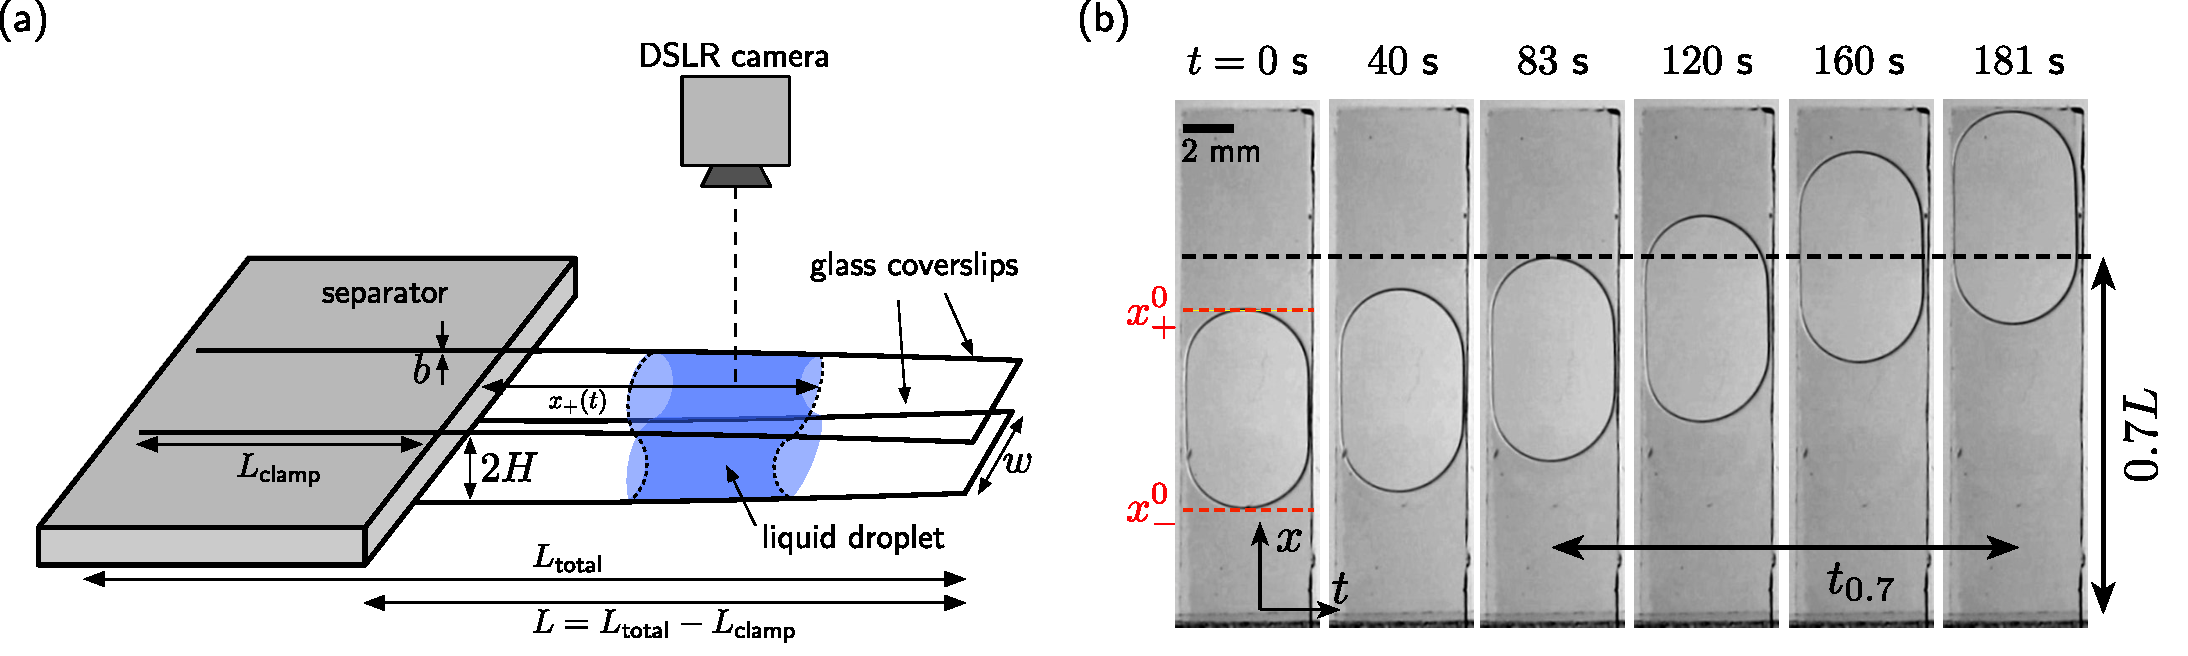
\includegraphics[width = \textwidth]{ExptSetup}
\caption{Experimental study of bendotaxis. (a) Schematic of the experimental setup consisting of a droplet in a flexible channel of undeformed wall separation $2H$, width $w$, and length $L$. We track the leading meniscus, located a distance $\xright(t)$ (measured along the centreline of the channel), during the experiment. (b) Top view of an example experiment with a V50 silicone oil droplet of volume $18~\si{\micro}$L. Here, $2H = 310$~$\si{\micro}$m, $L = 18$~mm, $w = 5$~mm,  and $b = 300$~$\si{\micro}$m. The scale bar indicates $2$~mm. The quantity $t_{0.7}$ is the time taken between $\xright = 0.7L$ and $\xright = L$, which corresponds to the time between the third and sixth images here.}
\label{fig:Ch3:ExptSetup}
\end{figure}
\subsection{Channel fabrication}\label{S:Ch3:ExperimentalSetup:Manufacture}
The experimental setup is shown in Figure~\ref{fig:Ch3:ExptSetup}.  To fabricate the channel, we cut two sections of borosilicate glass cover slips to a width $w$ from larger cover slips of length $L_{\text{total}}$. These coverslip sections were first treated (see below) before being clamped either side of a rigid separator of thickness $2H$ over a length $L_{\text{clamp}}$, to create an open-ended channel of length $L = L_{\text{total}} - L_{\text{clamp}}$ and half-thickness $H$.

%Why do we need to control tapering and how did we control it
Since the liquid motion is driven by a droplet induced tapering, we were careful to ensure that the channel has as little intrinsic tapering as possible. Intrinsic tapering is known to drive droplet motion, as studied by~\cite{Renvoise2009EPL} and~\cite{Reyssat2014JFM}, and including it here would interfere with the self-induced droplet motion of interest. To minimise intrinsic tapering, we clamped the channel walls over a length at least as long as the length of the resulting channel, i.e.~$L \lesssim L_{\text{clamp}}$ (Figure~\ref{fig:Ch3:ExptSetup}(a)).

\subsection{Channel wall treatment}\label{S:Ch3:ExperimentalSetup:WallTreatment}
The coverslips that make the channel walls were treated to minimize dissipation arising from dynamic contact angle effects and contact line pinning. As we shall see in the following chapter, the dynamics of bendotaxis is highly sensitive to contact angle hysteresis, which we have not yet included in our model. (In addition, recent studies of droplet dynamics in tapered channels by~\cite{Prakash2008Science} and~\cite{Bush2010AdvCollIntsci} have demonstrated how droplet motion can be arrested completely by contact angle hysteresis.)

We used two different treatments on the coverslips, which are described briefly here (full details can be found in Appendix~\ref{Appendix:Ch3:SurfaceCoating}). In one set of experiments, the glass was treated (prior to the channel fabrication) to render it a slippery lubricant-infused porous surface (SLIPS). Briefly, this treatment involves introducing a porous matrix to the surface of the coverslips, into which a lubricating silicone oil is impregnated. The result is an intrinsically smooth surface with no contact line pinning, since droplets of silicone oil subsequently introduced onto it share an interface only with the lubricant~\citep{Wong2011Nature}.

In the second set of experiments, the channel walls were pre-wetted with the same liquid as was used for the subsequent experiments in that channel. This treatment took place after the channel had been assembled. We ensured that the prewetting layer was sufficiently thin that liquid entrained during the experiment did not significantly alter the droplet's volume (Appendix~\ref{Appendix:Ch3:SurfaceCoating}).

%why use SLIPS vs why use prewetting. SLIPS: no hysteresis but do introduce dissipation in underlying film. Prewetting - ease.
The advantage of using SLIPS treated, rather than pre-wetted, coverslips for the channel walls is that this treatment guarantees low contact angle hysteresis and contact line dissipation.  The SLIPS treatment is, however, relatively resource intensive (by comparison with the pre-wetting treatment) and introduces another source of dissipation not accounted for by our model, namely viscous dissipation in the lubricant layer~\citep{Keiser2017SoftMatter}.

We find no difference between the SLIPS and pre-wetting treaments in our experimental data (Appendix~\ref{Appendix:Ch3:SurfaceCoating}). We interpret this agreement as evidence that contact line dissipation is negligible in the pre-wetting case, and lubricant dissipation is negligible in the SLIPS case. Henceforth, we shall not distinguish between the two cases.

\subsection{Experimental protocol}\label{S:Ch3:ExperimentalSetup:Performing}
Before the experiment began, a light spacer of thickness $2H$ was introduced to separate the free ends of the channel -- this allowed us to control the time at which the experiment begins. A liquid droplet of volume $\Omega$ was introduced close to the centre of this `doubly-clamped' channel using a micropipette with a narrow syringe tip (diameter 250~$\si{\micro}$m) attached. After deposition, the droplet sits at (what will become) its initial position.

Note that the clamped-clamped channel did experience a deformation in response to the presence of a droplet being introduced, but this deformation was relatively small. To justify this, we consider the limit of small droplets (which, as we shall see, predicts the dynamic behaviour of finite size droplets reasonably well). As demonstrated in Appendix A.3 of Chapter 2, a clamped-clamped channel does experience a deformation when a droplet is introduced but it is relatively small -- the maximum deformation is
\begin{equation}
\frac{\nu V H}{192} = \frac{\gamma \cos \theta_e L^3  \Delta X}{192 B H^2} H
\end{equation}
We have $\gamma \cos \theta_e L^3 \Delta X/(192 B H^2) < 0.02$ in all of our experiments: the channel deformation in the clamped-clamped state is never more than (approximately) 2\% of the channel half-width.

More important is the time scale of motion of a droplet in the clamped-clamped channel: in Appendix A.3 of Chapter 2, we also showed that, for a small droplet close to the centre of the channel, this time scale of droplet motion is
\begin{equation}
T = \frac{48 \mu B H}{\gamma^2 \cos^2 \theta_e \Delta X L},
\end{equation}
which is significantly longer ($\mathcal{O}$(10~minutes)) than the time spent in the clamped-clamped state ($\mathcal{O}$(10~seconds)). It is therefore reasonable to neglect any motion in the doubly clamped state, and, in particular, to assume that the droplet's position when it is deposited in the clamped-clamped configuration is the initial condition in the subsequent experiment.

The droplet was photographed in the clamped-clamped configuration using a DSLR camera (Nikon D700) mounted above the experiment. This image (and images of the subsequent experiment) have a resolution $1920\times1080$ pixels, with a typical spatial resolution of $0.03$~mm per pixel. Using this image, we determined $x_{\pm}(t = 0)$, the initial positions of the menisci -- measured along the centreline of the channel -- and thus the droplet length $\Delta X = \xright(t = 0) - \xleft(t = 0)$ and the relative volume $V = \Delta X /L$. To improve the contrast of the menisci, which appear as dark outlines, in images taken from above (Figure~\ref{fig:Ch3:ExptSetup}(b)), we lit the experiment from below (the curved interfaces at the menisci refract the light).

Droplets were heterogeneous in the third spatial direction (the direction that is not included in the model of Chapter 2, see Figure~\ref{fig:Ch3:ExptSetup}(b)) and the meniscus positions are measured at the droplet's longest point, so $V$ is an overestimate of the relative volume: $V = \Delta X/L > \Omega/(2H Lw)$. (The latter measure of relative volume was not used because there is large uncertainty in the actual amount of liquid that enters the channel.) Another important consequence of this heterogeneity is the presence of an interfacial curvature in the third spatial dimension (Figure~\ref{fig:Ch3:ExptSetup}(b)). However, this curvature, $\kappa_2 \sim L/w^2$, was relatively small in comparison with the curvature $\kappa_1 \sim 1/H$ of interest, for all parameter values considered.

When the spacer was removed, the droplet moved spontaneously towards the free end of the channel. The experiment was lit brightly from below and photographed from above with the same camera as described for determining the initial condition. The camera recorded one image every second. When the droplets reached the free end, we typically observed a small retreat of the rear `$-$' meniscus, after which the droplet remains stationary; the experiment concluded after the droplet had sat stationary (measured by eye) for $30$~s. Afterwards, the channel was disassembled and the wall thickness $b$ and spacer thickness $2H$ were measured with digital callipers (as a result, each experiment required a new channel to be fabricated).

As mentioned, the menisci are clearly visible as dark outlines in the images taken during the experiment (Figure~\ref{fig:Ch3:ExptSetup}(b)). A Canny edge detection algorithm~\citep{Canny1987} incorporated into a custom image analysis code written in
\textsc{matlab} was used to determine the outline of the droplet in the images taken during the experiment. Using the length of the channel to determine the spatial resolution of the images, we inferred from these outlines the meniscus trajectory $\xright(t)$ in each experiment.

Finally, to determine the effects of evaporation, several experiments were left in their `final' configuration overnight. No observable change in size or position had occurred by the next morning. This is consistent with our modelling assumption that evaporation is negligible.

\subsection{Parameter study}\label{S:Ch3:ExperimentalSetup:ParameterStudy}
%Describe ensemble
We performed the bendotaxis experiment 142 times in total. The liquid viscosity $\mu$, channel length $L$, channel thickness $2H$, droplet volume $\Omega$, and coverslip thickness $b$ were systematically varied across these experiments. The channel width $w = 5\pm0.5~\si{m\meter}$ and liquid--vapour interfacial tension $\gamma $ (see below) were held constant across the experiments. This channel width $w$ was the smallest we can reliably achieve -- cover slips typically fractured when cut to widths narrower than this (it is desirable to minimise the channel width $w$ as this reduces the influence of flow and cross-sectional volume variations in the spatial direction not accounted for by our model).

%Go through variation in each parameter: liquid viscosity
For each experiment, we used silicone oil (Sigma-Aldrich, USA) as the droplet liquid. We used silicone oils V50, V100, V350, and V500 with dynamic viscosities $\mu  = 48, 96, 336, 480~\si{\pascal~\second} \pm 5\%$ respectively (note that we calculate the dynamic viscosity as the product of the kinematic viscosity and density, whose values are provided by the manufacturer). These liquids have the same surface tension coefficient, $\gamma = 22 \pm 1~\si{m\newton}~\si{\meter}^{-1}$ (also provided by the manufacturer). Owing to the channel wall treatment, the silicone oil droplets share an interface only with the (lubricating) silicone oil and thus perfectly wet the channel walls ($\theta_e \approx 0$), but crucially form a capillary bridge with well-defined menisci.

Droplet volumes $\Omega$ in the range $10 \leq \Omega \leq 25 \pm 0.5~\si{\micro}\si{\liter}$ were used.

Each of the coverslips (Agar Scientific, UK) has a fixed length $L_{\text{total}} = 64~\si{\milli\meter}$; the channel length is varied in the range $14 \leq L \leq 30 \pm 0.25~\si{\milli\meter}$ by adjusting the clamped length, $L_{\text{clamp}}$. Whilst it would be desirable to probe a larger range of channel lengths (recall that our theory predicts sensitive dependence on $L$ through the bendability $\nu \sim L^4$), the upper bound on the channel length was chosen so that all configurations have a  pressure gradient contribution from gravity (defined in \S2.1) that is less than 10\% of the total pressure gradient. In addition, longer channels are more likely to have walls touch during the motion (at which point our theory breaks down). Finally, for channels with $L < 14~\si{\milli \meter}$, we observe that droplets do not occupy a significant portion of the channel and are pancake shaped; for these droplets, a two-dimensional theory is inadequate.

The separator, which sets the thickness of the channel, is fabricated by adhering two or more glass coverslips together. Using this method we achieved channel thicknesses  $310 \leq 2 H_0 \leq 630 \pm 5~\si{\micro}\si{\meter}$. (Note that each spacer is measured individually using a digital micrometer as the thickness of the adhesive layer used in fabricating the spacer is not known a priori).

We used three different thicknesses of coverslip (labelled no.~$1,1.5,$ and $2$ by the manufacturer) giving channel wall thicknesses in the range $160 \leq b \leq 310 \pm 5~\si{\micro}\si{\meter}$. (Note that if there is a difference in the measured values of $b$ between the upper and lower wall, we take the mean of the two values.)

With these parameter values, we achieve a large variation in the elasto-capillary number, $0.16 \leq \nu \leq 8$, as well as relative volumes in the range $0.20 \leq V \leq 0.51$. The combination of these results in almost two orders of magnitude variation in $\nu V$,  $0.24 \leq \nu V \leq 20$.

\section{Results}
\begin{figure}[h!]
\centering
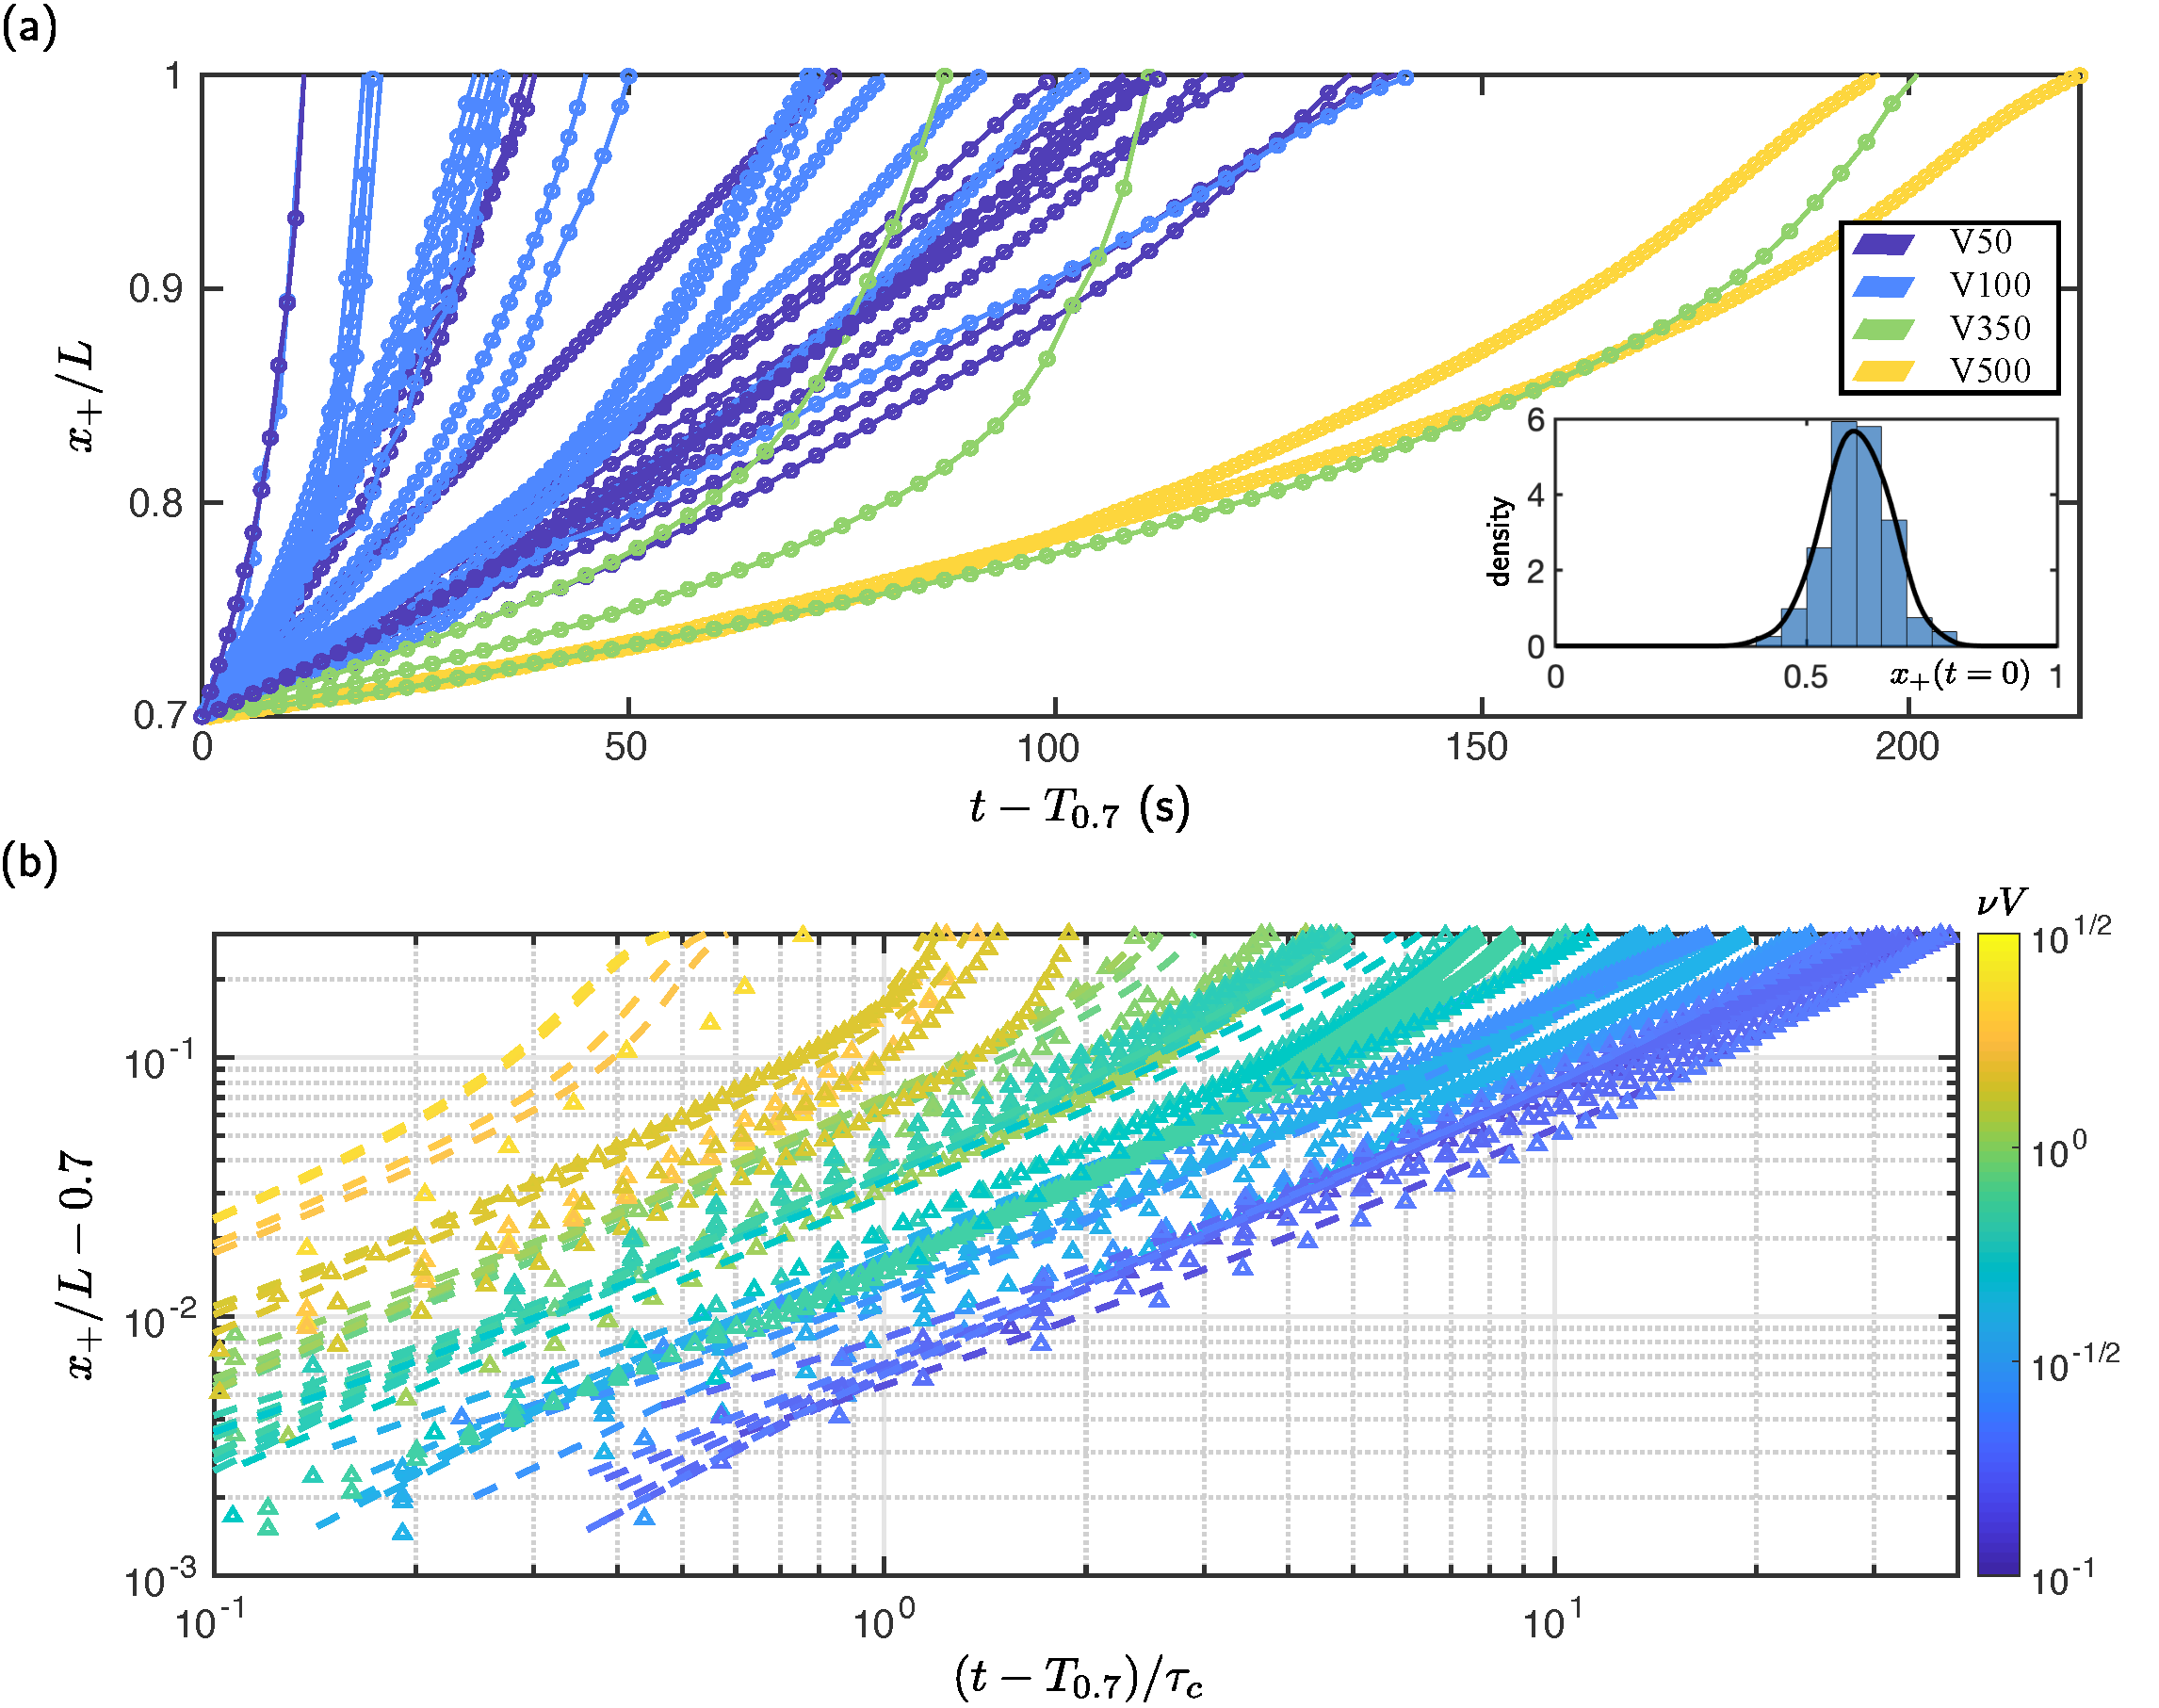
\includegraphics[scale=0.39]{ExptsFigV3}
\caption{(a) Trajectories of the meniscus displacement away from $t = T_{0.7}$, at which point $\xright = 0.7L$. Each curve corresponds to an individual experiment (which has a unique value of $T_{0.7}$). Circles indicate experimental data, obtained at 1~s intervals, connected by a spline to facilitate distinction between individual experiments. The legend indicates the type of silicone oil (and hence droplet viscosity) used in each experiment. Inset: histogram (blue boxes) and kernel density estimate (black line) of the initial conditions $\xright(t=0)/L$ in all 142 experiments. (These plots are scaled so that their total area is unity.) (b) Plot of the (displacement) trajectories shown in (a) as a function of dimensionless time on logarithmic axes (to facilitate identification of distinct trajectories). Triangles indicate experimental data and dashed curves indicate numerical solutions of the model equations (presented in \S2.2) using parameter values corresponding to the experiment. Points (both experimental and numerics) are coloured according to the value of $\nu V = BH^2 / (|\gamma \cos \theta_e|\Delta X L^3)$.}\label{fig:Ch3:ExptRawAndScaledTraces}
\end{figure}


\subsection{Raw results}
After image processing, each experiment yields a meniscus trajectory $\xright(t)$ with initial condition $\xright(0)$. Standardizing of initial conditions is difficult (it relies on the accuracy of inserting the droplet by hand), so we end up with a broad range of initial droplet positions $0.42 <\xright(t = 0)/L < 0.76$ with mean 0.6 and standard deviation 0.06 (the inset in Figure~\ref{fig:Ch3:ExptRawAndScaledTraces}(a) contains a plot of the kernel density estimate~\citep{Sheather2004StatSci} of $\xright/L$).

We do not directly compare experimental trajectories, as their behaviour is obfuscated by this difference in initial condition. Instead, we consider shifted trajectories:  we choose a point $0 < p < 1$ and determine the time, $T_p$, at which this trajectory passes $p$. We then define the shifted time $\tilde{t} = t - T_p$. We also consider the dimensionless displacement $\xright/L - p$, rather than the raw meniscus position. (Note that $T_p$ is related to the dimensional form of the quantity $t_f$ -- the time between the events $\xright/L = f$ and $\xright = 1$ --  by $T_f + t_f = t_{\text{total}}$, where $t_{\text{total}}$ is the time taken for the droplet to pass from its initial position to the end at $x = L$.)

Figure~\ref{fig:Ch3:ExptRawAndScaledTraces}(a) contains a plot of the trajectories $\xright(t)/L -  0.7$ (i.e.~taking $p = 0.7$ in the above definition). The data shown in this figure are only for those experiments with initial droplet positions $0.6L < \xright(t = 0) <0.65L$; this restriction ensures that only a manageable set of data (38 out of 142 total experiments) is presented. (Note that this restriction is somewhat arbitrary -- we could equally have taken $0.5L < \xright(t = 0) <0.55L$, for example -- but the particular choice we have made does cover the extremes of the parameter space described in the previous section.)

The trajectories demonstrate the large variation in dynamic behaviour which can be achieved by varying the experimental parameters. For example, the slowest moving droplet takes an order of magnitude longer to move from $\xright/L = 0.7$ to $\xright/L = 1$ (approximately $220$~s for the slowest moving droplet versus approximately $12$~s for the fastest). As expected, the viscosity plays a key role: the trajectories corresponding to high viscosity droplets (yellow and green trajectories in Figure~\ref{fig:Ch3:ExptRawAndScaledTraces}(a)) generally take much longer to traverse the final 30\% of the channel than the relatively low viscosity droplets (blue trajectories in Figure~\ref{fig:Ch3:ExptRawAndScaledTraces}(a)). The trajectories also indicate that droplets accelerate as they move along the channel, as the model developed in previous chapter predicts.

For a more detailed comparison between the model and experimental trajectories, we plot in Figure~\ref{fig:Ch3:ExptRawAndScaledTraces}(b) the trajectories as a function of dimensionless time (non-dimensionalized with the capillary time scale $\tau_c = \mu L^2 / (|\gamma \cos \theta_e| H)$). By plotting in this way, we are able to identify a strong dependence of the dynamic behaviour on the quantity $\nu V = BH^2 / (|\gamma \cos \theta_e|\Delta X L^3)$, which was identified as being important in the scaling argument in \S2.1. Those experiments corresponding to low $\nu V$ take a long time, relative to the capillary time scale (and vice versa for high $\nu V$). We postpone any detailed assessment of experimental dependence on $\nu V$ until the following subsection. 

Alongside each experimental trajectory, we plot in  the prediction of the full model for the appropriate parameter values, obtained using the numerical scheme described in \S2.2 (Figure~\ref{fig:Ch3:ExptRawAndScaledTraces}(b)). In each case, we use the initial conditions from the corresponding experiment. We see reasonable agreement between the numerical solutions and the experimental trajectories, and also that the spread of data -- the difference in time taken between the (relatively) fastest and slowest droplets --  is consistent between experiment and numerics, as is the shape of the trajectories.

Note that the numerical solutions typically overestimate the speed at which the droplets move along the channel (this is most pronounced in the case of large $\nu V$,  the yellow trajectories in Figure~\ref{fig:Ch3:ExptRawAndScaledTraces}(b)); these deviations are in the direction we expect -- neglecting the curvature $\kappa_2$, overestimating the droplet volume and ignoring contact line dissipation, would  each act to slow the droplet down.

%some segue to introducing the dynamic proxy?

\subsection{A proxy for the dynamics}
\begin{figure}[h]
\centering
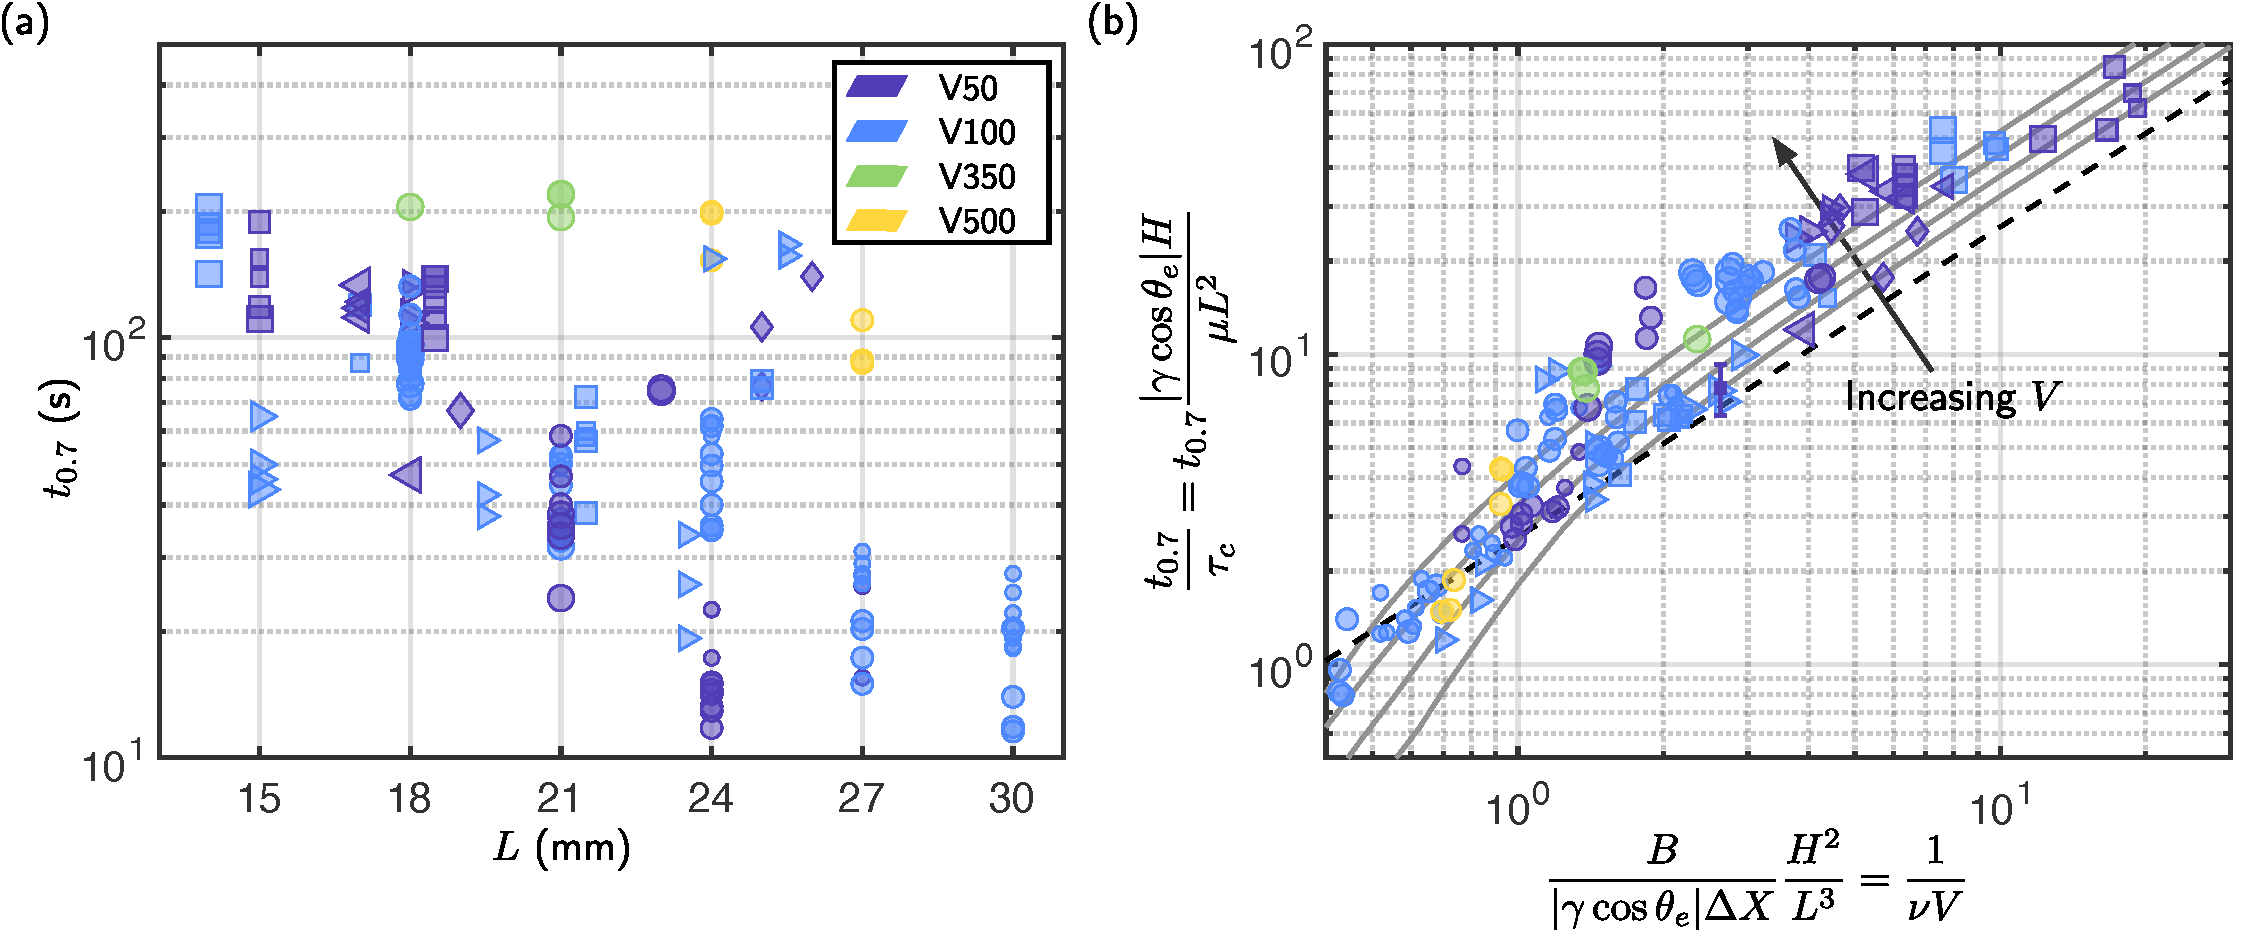
\includegraphics[width = \textwidth]{tpt7_both}
\caption{(a) Raw experimental measurements of $t_{0.7}$ for different channel lengths. The legend indicates the silicone oil used (and hence the viscosity, see main text). Different shapes encode channel wall separation as follows: $2H = 310~ \si{\micro \meter}$ (right triangle), $360 \si{\micro \meter}$ (left triangle), $430 \si{\micro \meter}$ (square),$ 540 \si{\micro \meter}$ (circle),$ 630 \si{\micro \meter}$ (diamond). The size of each point encodes the approximate fraction of the channel taken by the droplet ($V = \Delta X /L$), with bins corresponding to $V = 0.25, 0.25 \leq V < 0.35, 0.35 \leq V < 0.45$, and $V \geq 0.45$. (b) Collapse of the experimental data when rescaled according to~\eqref{E:Ch3:ScalingFunctionalForm_asymptotic}. A single set of error base extends one standard deviation away from a particular data point, computed from 20 measurements (see Appendix~\ref{Appendix:Ch3:SurfaceTreatment:Comparison}). Solid curves shown results from numerical solutions of the equations governing the model. Also plotted as a dashed line is the asymptotic result~\eqref{E:Ch3:ScalingFunctionalForm_asymptotic}, valid for $V \ll 1$ (corresponding to the upper right corner of this plot).}\label{fig:Ch3:RawT23}
\end{figure}

We have seen that the shape of the trajectories is well predicted by the theory. To allow a more robust comparison between the mathematical model developed in the previous chapter and the myriad experimental data (the data plotted in Figure~\ref{fig:Ch3:ExptRawAndScaledTraces} covers approximately 25\% of the the total), we re-introduce $t_f$, the time taken for the droplet to move between $\xright/L = f$ and $\xright / L = 1$. This quantity is a useful proxy to describe the dynamic behaviour throughout the experiment.

%very explicitly: why is t_f better than the full trace
There are two main benefits to considering the quantity $t_f$, rather than the full trajectories. Firstly, we have a single value of $t_f$ per experiment, vastly reducing the amount of data to be presented. Secondly, $t_f$ is approximately independent of the initial conditions and, as a result, removes the need to shift the time origin (this is in contrast to other proxies for the dynamic, such as mean square error between the numerical solution and experimental trajectory). Note, however, that by abstracting in this way, we remove any detail of \textit{how} the droplet gets from $\xright / L = f$ to $\xright / L = 1$ (other than how long it takes).

%what does t_f look like with respect to the model
Recall that the model developed in the previous chapter has three independent parameters: the dimensionless initial droplet position, $x_+(t = 0)/L$, the relative volume $V = \Delta X/ L$, and the bendability $\nu = \gamma \cos \theta_e L^4/(B H^2)$. In our model, however, $t_f/\tau_c$ is approximately independent of initial conditions; the model prediction of $t_f/\tau_c$ depends only on $\nu, V$,
\begin{equation}\label{E:Ch3:ScalingFunctionalForm}
\frac{t_{f}}{\tau_c} = F(\nu, V).
\end{equation}
In particular, the scaling argument in \S2.1 gives this functional dependence as
\begin{equation}\label{E:Ch3:ScalingFunctionalForm_scaling}
\frac{t_{f}}{\tau_c} \sim \frac{1}{\nu V}
\end{equation}
for $V \ll 1$ and $\nu \lesssim 1$. The asymptotic analysis for small droplets (see Appendix A of Chapter 2) gives the pre-factor
\begin{equation}\label{E:Ch3:ScalingFunctionalForm_asymptotic}
\frac{t_{f}}{\tau_c}  = \frac{6(1-f)}{f} \frac{1}{\nu V} \quad \text{as}~ V \to 0.
\end{equation}

%with the proxy, we can show all data and identify strong dependence on geometry which is hidden in the traces
In Figure~\ref{fig:Ch3:RawT23}(a) we present raw measurements of $t_{0.7}$ as a function of the channel length $L$. (Again, taking $f = 0.7$ is arbitrary but this value is sufficiently far from unity to allow a significant portion of the motion to be considered sufficiently. Experiments with $\xright(t =0) > 0.7L$ are then discounted of course, but less than 10\% of the experiments fall into this category.) Plotting the data against the channel length $L$ reveals a strong dependence of the dynamic behaviour on the channel length, which was not visible before. For example, droplets in channel with length $L = 30$~mm take an order of magnitude less time to traverse the final 30\% than droplets of the same viscosity in channels of length $L = 18$~mm.

Rescaling the data according to~\eqref{E:Ch3:ScalingFunctionalForm_scaling} provides a reasonable collapse (Figure~\ref{fig:Ch3:RawT23}(b)). For moderate to large values of the abscissa in Figure~\ref{fig:Ch3:RawT23}, we observe the scaling~\eqref{E:Ch3:ScalingFunctionalForm_scaling}. However, at smaller values of the abscissa (larger $V$), the linear scaling appears to break down.

We also include in Figure~\ref{fig:Ch3:RawT23}(b) curves corresponding to numerical solutions of the model equations for $V = 0.2, 0.3, 0.4, 0.5$ (i.e.~spanning the experimental range). The curves are obtained by numerically solving the model equations repeatedly at fixed $V$; by varying $\nu$ the curves in Figure~\ref{fig:Ch3:RawT23}(b) are traced out. These numerical solutions indicate that the non-linearity observed in the experimental data at small values of $\nu V$ is a real feature of the model that is not captured by the simple scaling argument described in \S2.1. For these experiments, the assumption of small deformations is no longer valid, and droplets traverse the channel quicker than the scaling argument predicts. Physically, this corresponds to the non-linearity in the pressure difference -- which arises when channel deformations are significant -- overcoming the non-linearity in the channel permeability (the former will reduce $t_f$ relative to the small deformation case, while the latter will increase it).

We also note that the spread between the numerical results corresponding to the largest and smallest values of $V$ is comparable to that in the experiments,  suggesting that some of the discrepancy between experiments and the asymptotic prediction~\eqref{E:Ch3:ScalingFunctionalForm_asymptotic} is accounted for by the finite value of $V$.

\section{Summary}
In this chapter we have presented an experimental investigation of bendotaxis. Although the `bench top' experiments are relatively simple, they provide a robust test of the model developed in the previous chapter.

In these experiments, we focussed primarily on the case of wetting droplets and were careful to minimize contact angle hysteresis and contact line dissipation; in the following chapter we consider the effect of contact angle hysteresis on the dynamics of bendotaxis.

The numerically and experimentally obtained droplet trajectories have a similar shape, but the model systematically over-predicts the speed with which droplets will traverse the channel. This is consistent with the two dimensional nature of our model: both interfacial curvature and volume variations in the third spatial dimension -- which are not included in the model -- are expected to slow the droplet down.

We considered the time to traverse a portion of the channel as a proxy for the dynamic behaviour; introducing this proxy facilitated quantitative comparison of a large set of data and reduced sensitivity of the results to initial conditions, which are hard to standardise in experiments. The experimental data for the traversal time indicate that the small deflection result derived in \S2.3 describes the dynamics reasonably well, even when the droplet has finite volume. The deviations from the small droplet result -- the non-linearity associated with large channel deflections, and the finite drop size effects predicted by the model -- are represented in the experimental data.

%couple of paragraphs saying what we did and the main conclusions (it feels like quite a sudden end if not!)

%\begin{appendix}
\begin{subappendices}
\renewcommand{\thesection}{\Alph{section}}
\section{Surface treatments}\label{Appendix:Ch3:SurfaceCoating}
Before each experiment, the glass coverslips were first treated to reduce the amount of contact line pinning and contact angle hysteresis. In this appendix we describe in more detail the two  techniques used to treat the channel walls -- SLIPS treatment and pre-wetting -- as well as additional experiments to test whether there is any difference between the dynamic behaviour in SLIPS treated and pre-wetted  channels.

\subsection{SLIPS treatment}
To achieve a slippery lubricant-infused porous surface on the glass coverslips, we followed the procedure outlined by~\cite{Guan2017SoftMatter}. The target surface was first sprayed with a commercial superhydrophobic coating (Glaco Mirror Coat Zero, Soft 99, Japan), which was then left to dry in ambient conditions. To ensure a robust coating, each target surface was sprayed three times; after the first two applications the surface was left to dry for 30 minutes, whilst after the third, the surface was left to dry for 24 hours, allowing the isopropanol in the spray to completely evaporate. This process left the target surface coated with hydrophobic nano-particles. By measuring the thickness of several coverslips before and after the nano-particle layer had been applied, we determined that the nano-particle layer thickness is negligible in comparison with that of the target surface.

After drying, the surfaces were dip coated in silicone oil (Sigma Aldrich, USA). The silicone oil penetrates the nano-particle structures, leaving a robust, lubricating coating on the target surface. Provided this lubricant is not displaced, droplets subsequently introduced onto the surface share an interface only with the lubricant; as a result, these droplets are highly mobile (the surface is ‘slippery’)~\citep{RuizGutierrez2017PRL}. The speed of withdrawal from the bath of lubricant was controlled using a linear actuator (M-229.26S Physik Instrumente, Germany) in conjunction with a motor controller (C-663 Mercury Step Controller, Physik Instrumente, Germany).

For surfaces to be used in experiments with wetting drops, we used V100 silicone oil as the lubricant, withdrawing at a speed of $100$~$\si{\micro}\si{\metre}~\si{\second}^{-1}$ (which has been reported to leave a lubricated layer of thickness approximately $3$~$\si{\micro}\si{\metre}$~\citep{Guan2017SoftMatter}). For the surface to be used in experiments with non-wetting drops we used V5 silicone oil as the lubricant, withdrawing at a speed $2$~mm~$\si{\second}^{-1}$. (In the non-wetting case, we used a lubricant with much lower viscosity to maximise the droplet:lubricant viscosity ratio and thus ensure that viscous dissipation occurs primarily within the droplet rather than in the lubricant layer~\citep{Keiser2017SoftMatter}).

The thickness of the lubricating layer follows a Landau--Levich scaling~\citep{Landau1942, Guan2017SoftMatter}; since the product of withdrawal speed and lubricant viscosity is equal in both wetting and non-wetting cases, the thickness of the lubricating layer should also be equal. This lubricant layer is sufficiently thin that it does not add significantly to the droplet volume, nor affect the droplet viscosity as liquid is entrained from the lubricating layer during the experiment.

\subsection{Pre-wetting}
To achieve a pre-wetted coating on the coverslips (without the addition of a porous surface), we introduced a liquid slug consisting of the same liquid as would be used for the subsequent experiments, at the clamped end of the channel. The whole assembly was tilted towards the (downward) vertical. As a result, the liquid drained under gravity to the free end, where any excess was removed.

The typical descent speed of the slug (which was controlled by varying the tilting angle, up to a maximum rotation of 90$\si{\degree}$) is $U \sim 10^{-2}~\text{m}~\text{s}^{\text{-1}}$, coats the channel walls with  layer of liquid with thickness $b_w \sim H (\mu U/\gamma)^{2/3}$~\citep{Landau1942}. The total volume of liquid deposited on each channel wall during the prewetting is therefore $V_{d} = Lwb_w$. For the highest viscosity liquid used in our experiments (V500 silicone oil with dynamic viscosity $\mu = 480~\si{\milli \pascal~\second}$ we calculate $b_w \sim 1~\si{\micro \metre}$ and $V_d \sim 1~\si{\micro \liter}$, which are relatively small in comparison with the range of droplet volumes ($10~\si{\micro \liter}$  $<\Omega <  25~\si{\micro \liter}$) and channel widths used. (Note that the calculation  $V_d \sim 1~\si{\micro \liter} $ provides an upper bound; the majority of experiments use V50 or V100 silicone oils, which have a  thinner pre-wetting layer.)


\subsection{Comparison between treatments}\label{Appendix:Ch3:SurfaceTreatment:Comparison}
\begin{figure}[t]
\centering
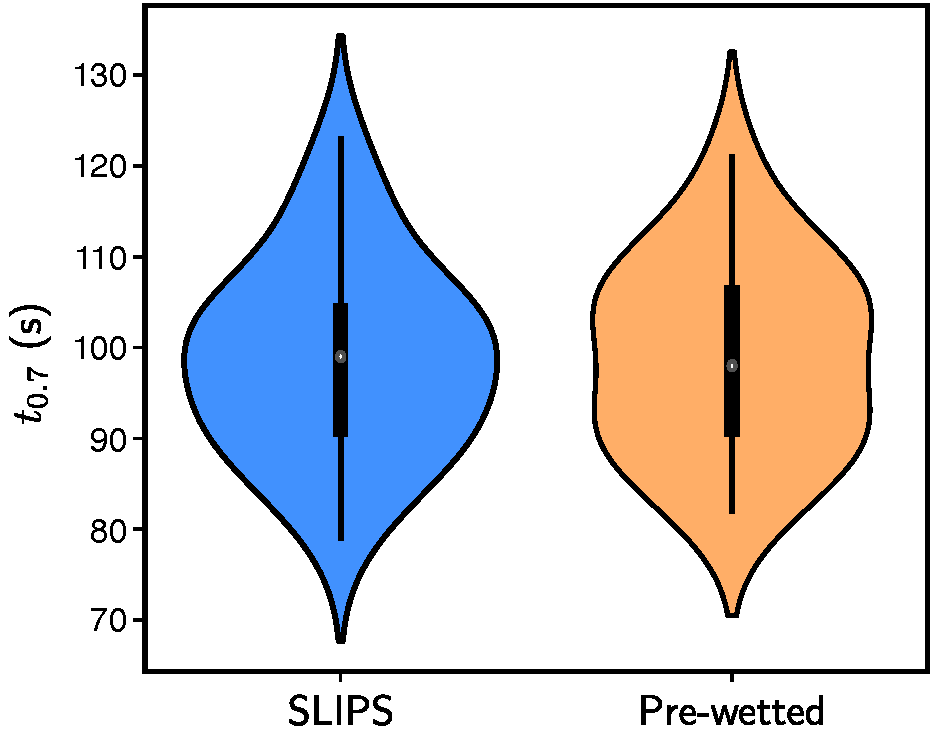
\includegraphics[scale=0.45]{SLIPS_vs_Prewet}
\caption{Violin plot of experimentally obtained values of $t_{0.7}$ for channels prepared with walls treated to achieve a SLIPS (left) and a pre-wetted surface (right). The data are obtained by performing the bendotaxis experiment repeatedly (25 times for SLIPS and 20 times for pre-wetted) using droplets V50 silicone oil droplets of volume $\Omega = 15~\si{\micro}$L in a channel with geometry as follows: $L = 27$~mm, $2H = 430~\si{\micro}$m, $w = 5$~mm, $b = 180~\si{\micro}$m. The mean values are $t_{0.7} = 98.85$~s and $t_{0.7} = 98.89$~s in the SLIPS and pre-wetted cases,
respectively, with standard deviations of $10.8$~s and $10.6$~s.  }\label{fig:Ch3:Appendix:SLIPSvsPrewet}
\end{figure}

To ascertain whether there was any difference between the dynamics of droplets in channels with pre-wetted and SLIPS walls, we performed the bendotaxis experiment repeatedly (25 times in a channel whose walls had been treated to be SLIPS, and 20 times in channels whose walls had been prewetted). The channel geometry was fixed as follows: $L = 27~\si{\milli \meter}$, $2H = 430~\si{\milli \meter}$, $w = 5~\si{\milli \meter}$, $b= 180~\si{\milli \meter}$. We used V50 silicone oil droplets of volume $\Omega = 15~\si{\micro \liter}$; small variations in thickness of the separator -- and hence channel thickness $2H$ -- as well as the volume of liquid we were able to get into the channel, meant that the relative volume $V$ varied in the interval $0.29 < V < 0.35$ (mean $0.32$, standard deviation $0.02$).

Figure~\ref{fig:Ch3:Appendix:SLIPSvsPrewet} shows violin plots~\citep{Hintze1998AmStat} of the values of $t_{0.7}$ for both cases; the kernel density estimates have very similar shapes about an identical mean $t_{0.7} = 98.9~
\si{\second}$. There is no significant difference in $t_{0.7}$ between the two treatments (SLIPS and pre-wetting) and we therefore conclude that the dynamic behaviour in our experimental study of bendotaxis is independent of the choice of surface treatment.

Note that we use the standard deviation in the SLIPS experiments as the error bar included in Figure~\ref{fig:Ch3:RawT23} and Figure~\ref{fig:Ch3:Appendix:tpt7_withNW}.


\section{Non-wetting configurations}\label{Appendix:Ch3:NonWetting}
In this appendix, we describe a suite of bendotaxis experiments performed in non-wetting configurations.
\subsection{Modifications to the experiment}
The experimental setup and protocol is identical to that described in \S3.1 except for two important changes.

Firstly, we used only a SLIPS treatment on the channel walls. We used V5 silicone oil as the lubricating liquid (rather than V50 in the wetting case); this lower viscosity lubricating liquid ensures that the dissipation in the lubricating layer is negligible in comparison with dissipation in the droplet (see Appendix~\ref{Appendix:Ch3:SurfaceCoating}).

The second modification is the use of a glycerol-water mix (GWM) for the droplets. The kinematic viscosity was measured
using a viscometer (Ametek Brookfield, UK) to be $30\pm5~\text{mm\textsuperscript{2}~s\textsuperscript{-1}}$. The density of the GWM was measured to
be $1.196~\text{kg~m\textsuperscript{-3}}$ using a densiometer (DMA 35, Anton Paar GmbH, Austria), from which we calculate a dynamic viscosity of $\mu = 35.9~\textsf{mPa~s}$. The air-liquid surface tension coefficient of the GWM was measured using the pendant drop method~\citep{Stauffer1965Pendant} to be $\gamma = 67~\textsf{mN~m\textsuperscript{-1}}$ (this value is in agreement with previously reported values~\citep{Takamura2012JPetSci}).

We measured the equilibrium contact angle of a $15~\si{\micro} \si{\L}$ droplet of GWM on a single, horizontal SLIPS infused with V5 silicone oil (i.e.~not within a channel) to be $\theta_e = 102\pm 1\si{\degree}$. This was determined by analyzing images taken with a microscope using the ImageJ contact angle plug-in~\citep{Schneider2012}. Errors in this calculation may be significant since the fit does not account for the lubricant skirt, which has a similar refractive index to the GWM. Further, it has been reported~\citep{Schellenberger2015SoftMatter} that microscopic contact angles on SLIPS can vary significantly from those obtained with the elliptic fit technique, while the use of an image of a droplet on a single SLIPS, rather than a channel makes the role of the skirt difficult to quantify. Using the same elliptical fit technique, we measured the advancing and receding contact angles of the droplet moving under gravity on a plate inclined by $1\si{\degree}$ to be $101.8\pm1.7\si{\degree}$ and $100.2\pm2.2\si{\degree}$, respectively.

\subsection{Results}
\begin{figure}[t]
\centering
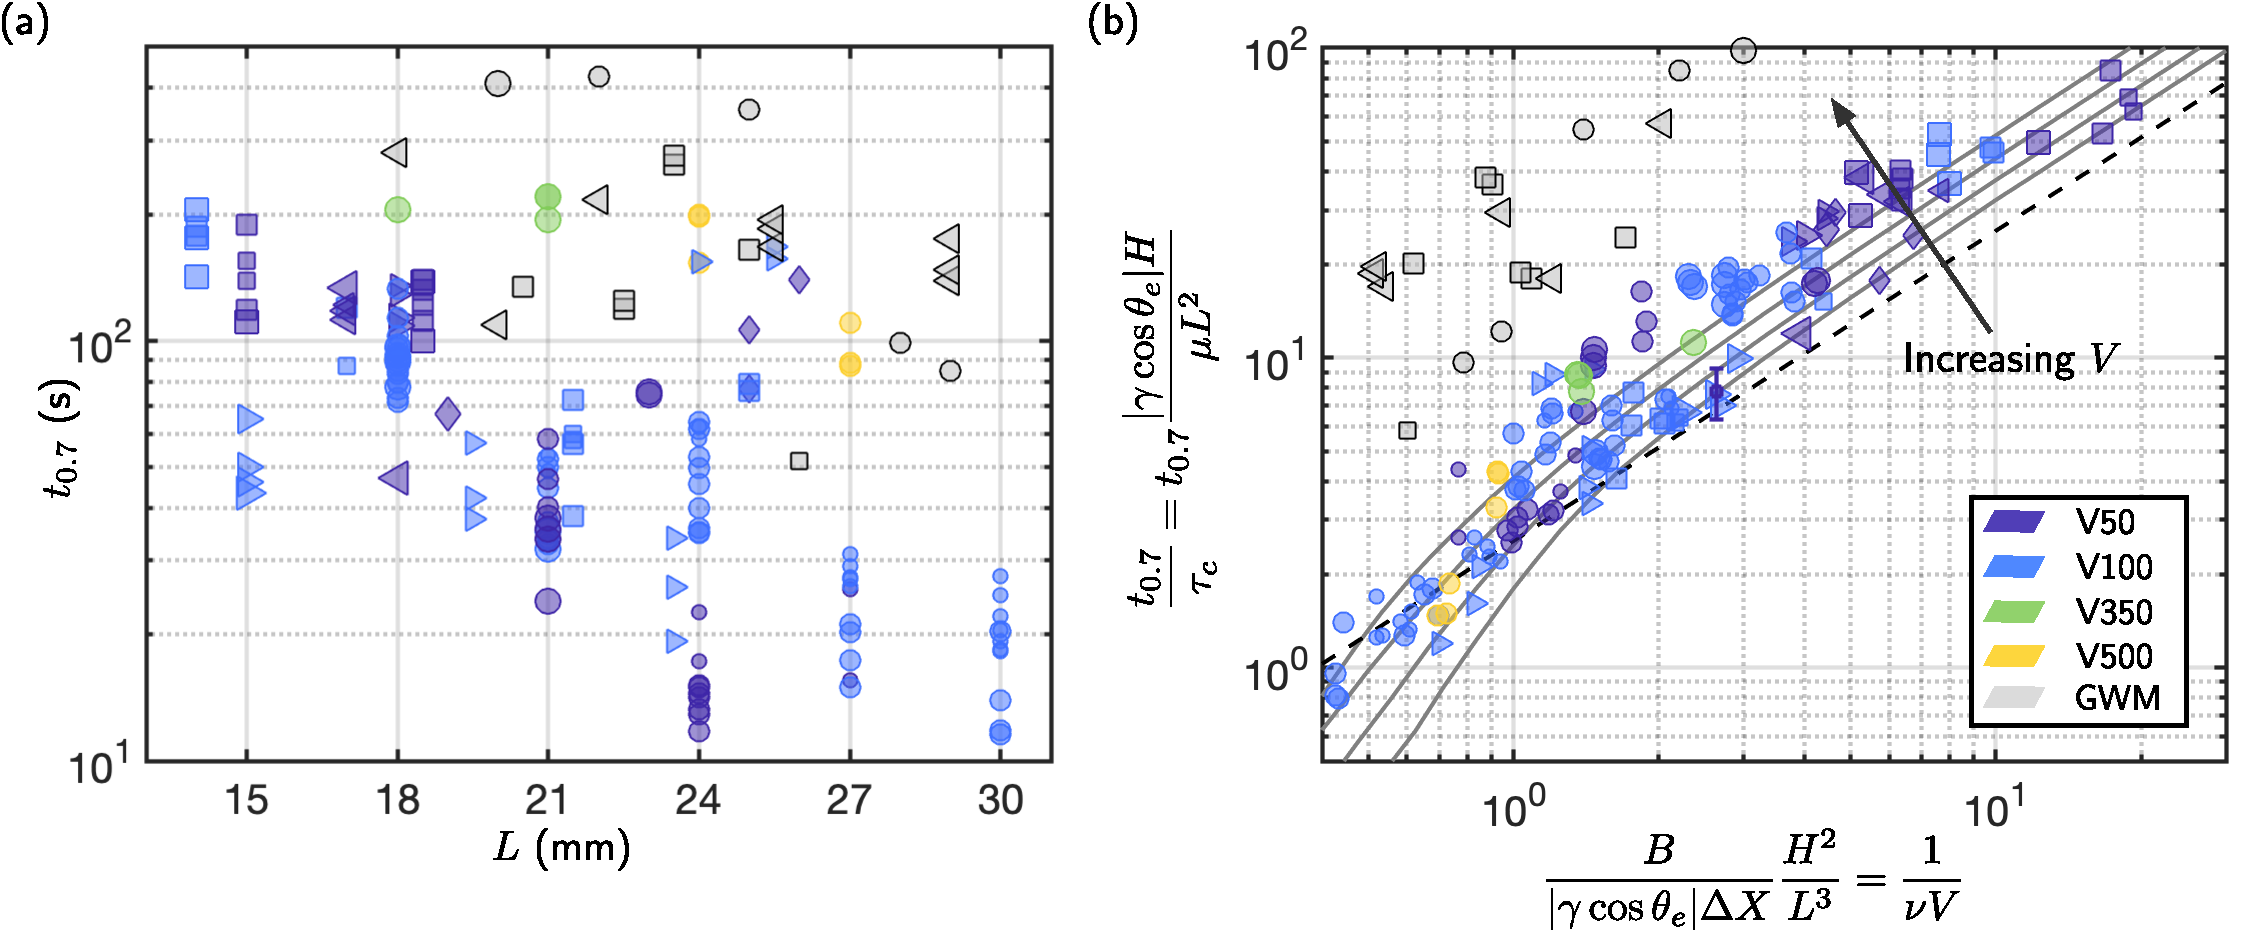
\includegraphics[width = \textwidth]{tpt7_both_with_NW}
\caption{ Raw experimental measurements of $t_{0.7}$ for different channel lengths. The legend in (b) indicates the liquid used (and hence the viscosity and wetting conditions, see main text). Shape and size of the data points encode channel width $2H$ and relative volume $V$, as in Figure~\ref{fig:Ch3:ExptSetup}. (b) Collapse of the experimental data when rescaled according to~\eqref{E:Ch3:ScalingFunctionalForm_asymptotic}. A single set of error bars extends one standard deviation away from a particular data point, computed from 20 measurements (see Appendix~\ref{Appendix:Ch3:SurfaceTreatment:Comparison}). Solid curves show results from numerical solutions of the equations governing the model. Also plotted is the asymptotic result~\eqref{E:Ch3:ScalingFunctionalForm_asymptotic} (including the corresponding pre-factor), valid for $V \ll 1$ (corresponding to the upper right corner of this plot).}\label{fig:Ch3:Appendix:tpt7_withNW}
\end{figure}

The non-wetting experiment was performed a total of 20 times, in channels whose geometry spanned the range described in \S\ref{S:Ch3:ExperimentalSetup:ParameterStudy}.

In Figure~\ref{fig:Ch3:Appendix:tpt7_withNW} we present the raw and rescaled measurements of $t_{0.7}$ from all experiments (i.e.~with both wetting and non-wetting experiments included). The raw experimental data indicate that droplets in non-wetting experiments generally take a longer time than droplets in wetting experiments to traverse the final 30\% of the channel, although the order of magnitude is similar (Figure~\ref{fig:Ch3:Appendix:tpt7_withNW}(a)). The dependence on the channel length is not visible for the data from non-wetting experiments, as it was for the wetting experiments.

When rescaled according to the scaling argument~\eqref{E:Ch3:ScalingFunctionalForm_scaling}, the data from non-wetting experiments show two families with a similar scaling trend but modified pre-factors. We believe that differences between the effective value of $|\gamma \cos \theta_e|$ between measurements made on a single SLIPS and experiments in a narrow channel may be responsible. In addition, droplets may be entirely coated, or `cloaked', by lubricant~\citep{McHale2019Langmuir}, in which case the air-liquid surface tension coefficient is not the correct one to use for the Laplace pressure; we believe that the two families correspond to whether the droplet is cloaked by lubricant or not. It is worth noting that the discrepancy in the pre-factor of the two families can be eliminated by a relatively small change in the effective contact angle of approximately $7\si{\degree}$ and $12\si{\degree}$, for the two families.

\end{subappendices}
